\chapter{Introduction}
% Context (1)
Data integration, cleaning and preparation are a part of the data science lifecycle. It is an exploratory process that takes a lot of effort, time and experiments.
Data engineers and data scientists in general spend between 80\% and 90\% of their time just on finding, collecting, integrating and cleaning datasets~\cite{80cleansurvey, dataintegration80}. The remaining 10\%-20\% are spent on model selection, training, scoring, and deployment.
% \textbf{Problems of dirty data:}
% Dirty data refers to data that contains erroneous or missing information.
It is a huge challenge in Databases (DB) and Machine Learning (ML) fields.
Both communities have been working on solutions of problems related to the dirty data~\cite{cleanml}. 
The ML community concentrates on impact of dirty data and noise on ML models~\cite{cleanml}.
It was studied that noise can have negligible effect on accuracy~\cite{processingsys, outperformstudy}, but ML models can also be sensitive to the dirty data, especially dirty labels~\cite{classificationnoisesurvey}.
The DB community's focus is on error detection and repairing~\cite{Hellerstein08quantitativedata, duplicatesstudy}.

% Problems (1-3) and Existing work (1)
\textbf{Data preparation and its challenges:}
Data cleaning is the process of removing faulty values from a dataset.
It consists of two steps: error detection and repair.
Error detection aims to identify errors, while error repair imputes/fixes flawed values using knowledge gathered from the input data. 
There are many existing techniques~\cite{duplicatesstudy, tdeexcel} and frameworks to clean the data such as HoloDetect/HoloClean~\cite{holodetect, RekatsinasCIR2017}, Raha/Baran~\cite{raha, baran}, BoostClean~\cite{boostclean}, AlphaClean~\cite{alphaclean}, ActiveClean~\cite{activeclean}. 
Existing techniques and frameworks are limited by additional user input such as hand-crafted constraints~\cite{bart}, or user manual labeling~\cite{raha, baran}.
For evaluation of data cleaning approaches the ground truth (GT) is required.
GT is not always available and is time-consuming to collect or create.
Sufficient data cleaning often requires an extra user input such as hand-crafted constraints~\cite{bart}, or user manual labeling.
Additionally, many datasets are private/confidential. 
Limited or even missing access to the data makes construction or acquisition of the ground truth extremely difficult. 
% While limited focus is made on scalable solutions that handle the cleaning of large datasets

\textbf{Data cleaning in ML pipelines}: 
Data cleaning is essential for the performance of ML models or databases.
It is part of the ML pipeline that aims to automate machine learning workflow. 
ML pipeline consists of several steps: data collection~\cite{LiDLMS2015}, data cleaning~\cite{raha, baran, RekatsinasCIR2017, holodetect, activeclean, alphaclean, cleanml}, feature extraction~\cite{ShahLKYK2021}, model training~\cite{RekatsinasCIR2017}, model debugging~\cite{SagadeevaB2021}, model evaluation~\cite{generalizing_confusion_matrix}, model visualization~\cite{NakandalaKP2019, CrottyGZBK2015, SimonyanVZ2013}, and model serving~\cite{OlstonFGHLLRR2017, Lee2018, WeiGZWCNOSR2018}.
Data preparation is a key step and obeys the garbage in, garbage out principle (GIGO).
GIGO is the concept that flawed input data produces nonsense output.

% Idea (1) and Contributions 
\textbf{Contributions:} 
This paper aims to create a tool for the distributed dirty data generation that can be used by the ML and DB communities. 
The high level list of contributions is:

\begin{itemize}
    \item A study of existing data cleaning tools and frameworks.
    \item Local and Spark distributed scaling that allows scales about the powers of single machines.
    \item Error extraction and techniques for error type detection between ground truth and dirty data.
    \item Data generation with configurable errors and error rates.
    \item Novel techniques to preserve the statistical properties of the input data while generating new data.
    \item Experimental evaluation of the data generator.
    % \item This paper, describing techniques and algorithms used.
\end{itemize}

Finally, this framework is a part of a larger project called WashHouse, a data cleaning for ML benchmark, that is designed to solve the problem of evaluation of data cleaning approaches, and the problem of the missing ground truth datasets.

% WashHouse scales clean and dirty versions of the dataset, preserving data and error distributions. 
% WashHouse extracts real error patterns from the dataset and scales data with configurable errors and error rates. 
% It covers eight real-world error classes (e.g., missing values, outliers).

% \begin{figure}[!b]
%     \centering
% 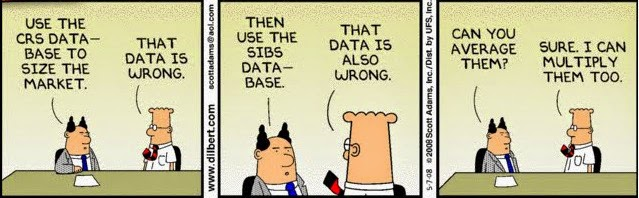
\includegraphics[width=\textwidth]{figures/Dilbert-Dirty.jpg}
%     \caption{On the details of calculating with dirty values}
%     \label{fig:dilbert}
% \end{figure}
